
\providecommand{\llsq}{\mathrel{\square}}%

\section{提升性质、弱分解系统与 Leibniz 闭性}\label{sec:weak-factorization-systems}

固定\trCategory{} $\mathcal{M}$ 中的两个箭头 $j$ 与 $p$，我们把任何形如
\begin{center}
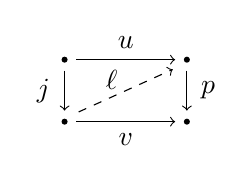
\begin{tikzpicture}[x=1.7em,y=1.6em]
  \fill (0,1.4) circle (1.1pt);
  \fill (2.6,1.4) circle (1.1pt);
  \fill (0,0) circle (1.1pt);
  \fill (2.6,0) circle (1.1pt);
  \draw[->] (0.25,1.4) -- (2.35,1.4);
  \node at (1.3,1.78) {$u$};
  \draw[->] (0,1.15) -- (0,0.25);
  \node at (-0.45,0.7) {$j$};
  \draw[->] (2.6,1.15) -- (2.6,0.25);
  \node at (3.05,0.7) {$p$};
  \draw[->] (0.25,0) -- (2.35,0);
  \node at (1.3,-0.4) {$v$};
  \draw[->,dashed] (0.3,0.22) -- (2.3,1.18);
  \node at (1.0,0.95) {$\ell$};
\end{tikzpicture}
\end{center}
的交换方块视作 $j$ 与 $p$ 之间的一个\trLifting{}问题，它经由构造一个提升——
一条使两个三角形都交换的对角态射 $\ell$——而得解。若 $j$ 与 $p$ 之间的每个%
\trLifting{}问题都有解，我们便说 $j$ 对 $p$ 具有\textbf{左\trLifting{}性质}%
（left lifting property），等价地，$p$ 对 $j$ 具有\textbf{右%
\trLifting{}性质}（right lifting property）。此时，我们采用富有暗示意味的
记号 $j\llsq p$ 来断言这一提升性质。

在抽象\trHomotopy{}论中，令人感兴趣的映射类时常由对另一类或一集映射的左或
右\trLifting{}性质来刻画。

\begin{definition}\label{def:lifting-classes}
设 $J$ 是\trCategory{} $\mathcal{M}$ 中的一个映射类。
\begin{itemize}
\item 记 $J\llsq$ 为 $\mathcal{M}$ 中对 $J$ 中每个态射都具有右\trLifting{}性质
  的映射组成的类。
\item 记 $\llsq J$ 为 $\mathcal{M}$ 中对 $J$ 中每个态射都具有左\trLifting{}性质
  的映射组成的类。
\end{itemize}
\end{definition}

\begin{example}\label{exa:isofibration-trivial-lifting}
第 1 章中的\cref{def:isofibration}与\cref{def:trivial-fibration}以对映射之集
\[ \{\Lambda^k[n]\hookrightarrow\Delta[n]\}_{n\ge 2,\,0<k<n}
   \cup\{\qcOne\hookrightarrow\qcInt\}
   \qquad\text{与}\qquad
   \{\partial\Delta[n]\hookrightarrow\Delta[n]\}_{n\ge 0} \]
的右\trLifting{}性质，分别刻画了\trQuasiCategory{}之间的\trIsofibration{}与%
\trTrivialFibration。
\end{example}

由右\trLifting{}性质刻画的映射自动满足各种如今或许已经眼熟的封闭性质。

\begin{lemma}\label{lem:right-lifting-closure}
由右\trLifting{}性质刻画的任何映射类 $J\llsq$ 都包含全部\trIsomorphism，并对
复合、\trProduct、\trPullback、\trRetract{}以及塔的\trLimit{}封闭。
\end{lemma}

在陈述中，「积」与「收缩」指称在\trCategoryOfArrows{}中构成的极限，而「拉回」
则是 $J\llsq$ 中的映射沿任一映射的拉回。「塔」指形状为 $\alpha^{\mathrm{op}}$ 的
图表，其中 $\alpha$ 是一个极限序数（极可能是 $\omega$）。

\begin{proof}
诸论证皆类似。例如，设 $q$ 是 $p\in J\llsq$ 的一个\trPullback。把下方左侧的%
\trLifting{}问题与下方右侧的\trPullback{}方块并置，便可求解 $j$ 对 $p$ 的复合%
\trLifting{}问题而得到虚对角态射 $\ell$，然后经由在\trPullback{}图式上由
$(v,\ell)$ 构成的\trCone，诱导出 $j$ 对 $q$ 的\trLifting{}问题的一个解 $s$：
\begin{center}
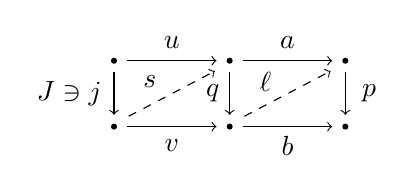
\begin{tikzpicture}[x=1.9em,y=1.7em]
  \fill (0,1.4) circle (1.1pt);
  \fill (2.2,1.4) circle (1.1pt);
  \fill (4.4,1.4) circle (1.1pt);
  \fill (0,0) circle (1.1pt);
  \fill (2.2,0) circle (1.1pt);
  \fill (4.4,0) circle (1.1pt);
  \draw[->] (0.25,1.4) -- (1.95,1.4);
  \node at (1.1,1.78) {$u$};
  \draw[->] (2.45,1.4) -- (4.15,1.4);
  \node at (3.3,1.78) {$a$};
  \draw[->] (0,1.15) -- (0,0.25);
  \node at (-0.85,0.7) {$J\owns j$};
  \draw[->] (2.2,1.15) -- (2.2,0.25);
  \node at (1.88,0.7) {$q$};
  \draw[->] (4.4,1.15) -- (4.4,0.25);
  \node at (4.85,0.7) {$p$};
  \draw[->] (0.25,0) -- (1.95,0);
  \node at (1.1,-0.4) {$v$};
  \draw[->] (2.45,0) -- (4.15,0);
  \node at (3.3,-0.4) {$b$};
  \draw[->,dashed] (0.28,0.22) -- (1.92,1.18);
  \node at (0.68,0.95) {$s$};
  \draw[->,dashed] (2.48,0.22) -- (4.12,1.18);
  \node at (2.88,0.95) {$\ell$};
  \node at (2.55,1.08) {$\scriptstyle\lrcorner$};
\end{tikzpicture}
\end{center}
于是 $q$ 对 $J$ 可提升，从而属于 $J\llsq$。
\end{proof}

由于\cref{lem:right-lifting-closure}的对偶，余完备\trCategory{}中的任何映射之
集都「胞腔式生成」一个更大的、具有同一左\trLifting{}性质的映射类。

\begin{definition}\label{def:cell-complex}
设 $J$ 是一个我们视作「基本\trCell{}」的映射之集。一个%
\textbf{$J$-胞腔复形}（$J$-cell complex）是一个作为 $J$ 中映射之余积的推出经
超限复合而构筑起来的映射：
\begin{center}
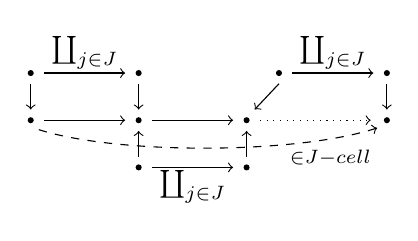
\begin{tikzpicture}[x=1.95em,y=1.55em]
  \fill (0,2.2) circle (1.1pt);
  \fill (2.0,2.2) circle (1.1pt);
  \fill (4.6,2.2) circle (1.1pt);
  \fill (6.6,2.2) circle (1.1pt);
  \fill (0,1.1) circle (1.1pt);
  \fill (2.0,1.1) circle (1.1pt);
  \fill (4.0,1.1) circle (1.1pt);
  \fill (6.6,1.1) circle (1.1pt);
  \fill (2.0,0) circle (1.1pt);
  \fill (4.0,0) circle (1.1pt);
  \draw[->] (0.25,2.2) -- (1.75,2.2);
  \node at (1.0,2.66) {$\coprod_{j\in J}$};
  \draw[->] (4.85,2.2) -- (6.35,2.2);
  \node at (5.6,2.66) {$\coprod_{j\in J}$};
  \draw[->] (0,1.95) -- (0,1.35);
  \draw[->] (2.0,1.95) -- (2.0,1.35);
  \draw[->] (4.6,1.95) -- (4.15,1.35);
  \draw[->] (6.6,1.95) -- (6.6,1.35);
  \draw[->] (0.25,1.1) -- (1.75,1.1);
  \draw[->] (2.25,1.1) -- (3.75,1.1);
  \draw[->,dotted] (4.25,1.1) -- (6.3,1.1);
  \draw[->] (2.0,0.25) -- (2.0,0.85);
  \draw[->] (4.0,0.25) -- (4.0,0.85);
  \draw[->] (2.25,0) -- (3.75,0);
  \node at (3.0,-0.46) {$\coprod_{j\in J}$};
  \node at (1.68,1.4) {$\lrcorner$};
  \node at (4.32,0.82) {$\urcorner$};
  \draw[->,dashed] (0.15,0.88) .. controls (1.6,0.3) and (4.9,0.3) .. (6.42,0.92);
  \node at (5.55,0.22) {$\scriptstyle\in J\text{-cell}$};
\end{tikzpicture}
\end{center}
\end{definition}

诸 $J$-胞腔复形组成的类 $J\text{-cell}$ 称为由映射之集 $J$ \trCell{}式生成。
由映射之集 $J$ \textbf{余纤维性生成}（cofibrantly generated）的映射类
$J\text{-cof}$，由那些作为这些映射之余积的推出的序列复合的收缩而得到的映射
组成。

\begin{definition}\label{def:weak-factorization-system}
\trCategory{} $\mathcal{M}$ 上的一个弱分解系统 $(\mathrm{L},\mathrm{R})$ 由
态射类 $\mathrm{L}$ 与 $\mathrm{R}$ 组成，使得
\begin{enumerate}[label=(\roman*)]
\item $\mathcal{M}$ 中每个态射都可分解为 $\mathrm{L}$ 中一个态射接 $\mathrm{R}$
  中一个态射：
\begin{center}
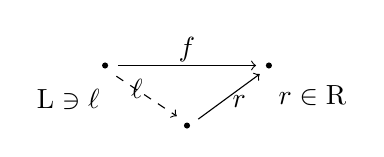
\begin{tikzpicture}[x=1.85em,y=1.55em]
  \fill (0,1.4) circle (1.1pt);
  \fill (3.2,1.4) circle (1.1pt);
  \fill (1.6,0) circle (1.1pt);
  \draw[->] (0.25,1.4) -- (2.95,1.4);
  \node at (1.6,1.78) {$f$};
  \draw[->,dashed] (0.22,1.15) -- (1.4,0.22);
  \node at (-0.72,0.62) {$\mathrm{L}\owns\ell$};
  \node at (0.62,0.85) {$\ell$};
  \draw[->] (1.82,0.15) -- (3.02,1.2);
  \node at (2.62,0.55) {$r$};
  \node at (4.05,0.7) {$r\in\mathrm{R}$};
\end{tikzpicture}
\end{center}
\item 类 $\mathrm{L}$ 与 $\mathrm{R}$ 彼此之间分别具有左、右\trLifting{}性质
  $\mathrm{L}\llsq\mathrm{R}$；也就是说，从 $\mathrm{L}$ 中一个映射到
  $\mathrm{R}$ 中一个映射的任何交换方块都有对角填充：
\begin{center}
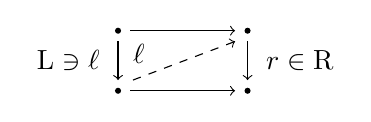
\begin{tikzpicture}[x=1.8em,y=1.55em]
  \fill (0,1.4) circle (1.1pt);
  \fill (2.6,1.4) circle (1.1pt);
  \fill (0,0) circle (1.1pt);
  \fill (2.6,0) circle (1.1pt);
  \draw[->] (0.25,1.4) -- (2.35,1.4);
  \draw[->] (0,1.15) -- (0,0.25);
  \node at (-1.0,0.7) {$\mathrm{L}\owns\ell$};
  \node at (0.42,0.85) {$\ell$};
  \draw[->] (2.6,1.15) -- (2.6,0.25);
  \node at (3.65,0.7) {$r\in\mathrm{R}$};
  \draw[->,dashed] (0.3,0.25) -- (2.35,1.15);
  \draw[->] (0.25,0) -- (2.35,0);
\end{tikzpicture}
\end{center}
\item 并且 $\mathrm{L}=\llsq\mathrm{R}$ 而 $\mathrm{R}=\mathrm{L}\llsq$。
\end{enumerate}
\end{definition}

作为\cref{def:weak-factorization-system}(iii) 的推论，弱分解系统的右类享有
\cref{lem:right-lifting-closure}的诸封闭性质，而左类则对对偶构造封闭。

在一对伴随\trFunctor{}在场时，提升性质可以转置。

\begin{lemma}\label{lem:adjunction-transposes-lifting}
在伴随在场时：
\begin{center}
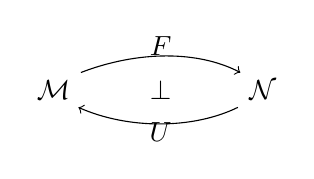
\begin{tikzpicture}[x=1.8em,y=1.5em]
  \node (M) at (0,0) {$\mathcal{M}$};
  \node (N) at (4.2,0) {$\mathcal{N}$};
  \draw[->] (0.55,0.42) .. controls (1.7,0.95) and (2.9,0.95) .. (3.75,0.42);
  \node at (2.15,1.05) {$F$};
  \draw[->] (3.7,-0.42) .. controls (2.8,-0.95) and (1.5,-0.95) .. (0.5,-0.42);
  \node at (2.15,-1.02) {$U$};
  \node at (2.15,0) {$\perp$};
\end{tikzpicture}
\end{center}
\begin{enumerate}[label=(\roman*)]
\item 下方左侧所示的 $\mathcal{N}$ 中\trLifting{}问题的解经转置可定义下方右侧
  所示的 $\mathcal{M}$ 中转置\trLifting{}问题的解：
\begin{center}
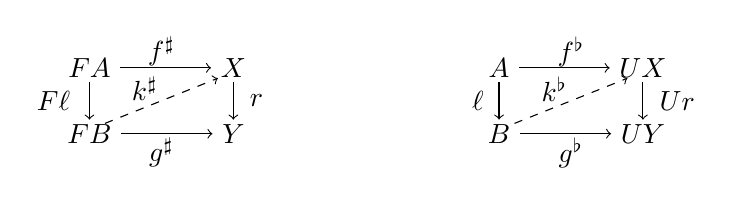
\begin{tikzpicture}[x=2.0em,y=1.7em]
  \node (FA) at (0,1.4) {$FA$};
  \node (X) at (2.6,1.4) {$X$};
  \node (FB) at (0,0) {$FB$};
  \node (Y) at (2.6,0) {$Y$};
  \draw[->] (FA) -- (X);
  \node at (1.3,1.74) {$f^{\sharp}$};
  \draw[->] (0,1.1) -- (0,0.3);
  \node at (-0.65,0.7) {$F\ell$};
  \draw[->] (2.6,1.1) -- (2.6,0.3);
  \node at (3.02,0.7) {$r$};
  \draw[->] (FB) -- (Y);
  \node at (1.3,-0.4) {$g^{\sharp}$};
  \draw[->,dashed] (0.28,0.22) -- (2.32,1.18);
  \node at (1.0,0.95) {$k^{\sharp}$};
  \node (A) at (7.4,1.4) {$A$};
  \node (UX) at (10.0,1.4) {$UX$};
  \node (B) at (7.4,0) {$B$};
  \node (UY) at (10.0,0) {$UY$};
  \draw[->] (A) -- (UX);
  \node at (8.7,1.74) {$f^{\flat}$};
  \draw[->] (7.4,1.1) -- (7.4,0.3);
  \node at (7.02,0.7) {$\ell$};
  \draw[->] (10.0,1.1) -- (10.0,0.3);
  \node at (10.62,0.7) {$Ur$};
  \draw[->] (B) -- (UY);
  \node at (8.7,-0.4) {$g^{\flat}$};
  \draw[->,dashed] (7.68,0.22) -- (9.72,1.18);
  \node at (8.4,0.95) {$k^{\flat}$};
\end{tikzpicture}
\end{center}
\item 若 $\mathcal{M}$ 带有弱分解系统 $(\mathrm{L},\mathrm{R})$ 而
  $\mathcal{N}$ 带有弱分解系统 $(\mathrm{L}',\mathrm{R}')$，则 $F$ 保持左类
  当且仅当 $U$ 保持右类：
  \[ \mathrm{FL}\subset\mathrm{L}'
     \quad\leftrightsquigarrow\quad
     \mathrm{R}\supset U\mathrm{R}'. \]
\end{enumerate}
\end{lemma}

\cref{def:weak-factorization-system}的诸分解式与 (ii) 全然无关，但我们仍针对
弱分解系统陈述这一结果，因为这正是它通常被应用的语境。
\begin{proof}
\cref{ex:prove-adjunction-transposes}。
\end{proof}

\cref{lem:adjunction-transposes-lifting}(ii) 定义了\textbf{弱分解系统的伴随}%
（adjunction of weak factorization systems）这一概念：这是配备弱分解系统的诸%
\trCategory{}之间的一对伴随\trFunctor，使得左\trAdjunction{}保持左类而右%
\trAdjunction{}保持右类。我们现在的目标是把这一概念推广到双变量\trAdjunction{}上，%
\footnote{对 $n$-变量\trAdjunction{}有一个类似的推广，可在 \cite[\S4]{bib26}
中找到。}后者由一个三元组的\trBifunctor{}给出：
\begin{rveq}\label{eq:two-variable-adjunction-functors}
\mathcal{V}\times\mathcal{M}\xrightarrow{\;\otimes\;}\mathcal{N},\qquad
\mathcal{V}^{\mathrm{op}}\times\mathcal{N}\xrightarrow{\;\{,\}\;}\mathcal{M},
\qquad
\mathcal{M}^{\mathrm{op}}\times\mathcal{N}\xrightarrow{\;\mathrm{hom}\;}\mathcal{V}
\end{rveq}
书写时所用的记号暗示着最常见的例子，并配备有一个自然\trIsomorphism
\[ \mathcal{N}(\mathcal{V}\otimes\mathcal{M},\mathcal{N})
   \cong\mathcal{M}(\mathcal{M},\{\mathcal{V},\mathcal{N}\})
   \cong\mathcal{V}(\mathcal{V},\mathrm{hom}(\mathcal{M},\mathcal{N})). \]

\trBifunctor{} $\otimes\colon\mathcal{V}\times\mathcal{M}\to\mathcal{N}$ 的
「推出积」定义了一个\trBifunctor{}
$\widehat{\otimes}\colon\mathcal{V}^{2}\times\mathcal{M}^{2}\to\mathcal{N}^{2}$；
当该\trBifunctor{} $\otimes$ 被称作「张量」时，我们把 $\widehat{\otimes}$ 称作
「\trLeibnizTensor」。「\trLeibnizCotensor」与「Leibniz hom」
\[ \widehat{\{,\}}\colon(\mathcal{V}^{2})^{\mathrm{op}}\times\mathcal{N}^{2}
     \to\mathcal{M}^{2}
   \qquad\text{与}\qquad
   \widehat{\mathrm{hom}}\colon(\mathcal{M}^{2})^{\mathrm{op}}\times\mathcal{N}^{2}
     \to\mathcal{V}^{2} \]
则对偶地定义，分别在 $\mathcal{M}$ 与 $\mathcal{V}$ 中使用拉回。

\begin{definition}[Leibniz 张量与余张量]\label{def:leibniz-tensor-cotensor}
给定取值于带推出\trCategory{}的\trBifunctor{}
$\otimes\colon\mathcal{V}\times\mathcal{M}\to\mathcal{N}$，$\mathcal{V}$ 中映射
$k\colon I\to J$ 与 $\mathcal{M}$ 中映射 $\ell\colon A\to B$ 的%
\trLeibnizTensor{}是 $\mathcal{N}$ 中由下方左侧的推出图式所诱导的映射
$k\widehat{\otimes}\ell$：
\begin{center}
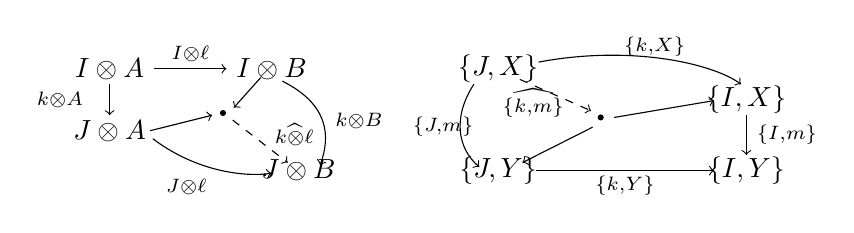
\begin{tikzpicture}[x=1.95em,y=1.6em]
  \node (IA) at (0,1.9) {$I\otimes A$};
  \node (IB) at (3.0,1.9) {$I\otimes B$};
  \node (JA) at (0,0.5) {$J\otimes A$};
  \fill (2.1,0.9) circle (1.1pt);
  \node (JB) at (3.5,-0.4) {$J\otimes B$};
  \draw[->] (IA) -- (IB);
  \node at (1.5,2.24) {$\scriptstyle I\otimes\ell$};
  \draw[->] (0,1.55) -- (0,0.85);
  \node at (-0.92,1.2) {$\scriptstyle k\otimes A$};
  \draw[->] (0.75,0.5) -- (1.9,0.85);
  \draw[->] (2.8,1.7) -- (2.3,1.02);
  \draw[->,dashed] (2.28,0.74) -- (3.3,-0.22);
  \node at (3.42,0.42) {$\scriptstyle k\widehat{\otimes}\ell$};
  \draw[->] (3.2,1.62) .. controls (4.05,1.1) and (4.1,0.4) .. (3.9,-0.28);
  \node at (4.62,0.72) {$\scriptstyle k\otimes B$};
  \draw[->] (0.8,0.32) .. controls (1.6,-0.42) and (2.5,-0.55) .. (3.0,-0.46);
  \node at (1.42,-0.78) {$\scriptstyle J\otimes\ell$};
  \node at (1.82,1.12) {$\lrcorner$};
  \node (JX) at (7.2,1.9) {$\{J,X\}$};
  \node (IX) at (11.8,1.2) {$\{I,X\}$};
  \fill (9.1,0.8) circle (1.1pt);
  \node (JY) at (7.2,-0.4) {$\{J,Y\}$};
  \node (IY) at (11.8,-0.4) {$\{I,Y\}$};
  \draw[->] (7.95,2.05) .. controls (9.7,2.45) and (11.2,2.0) .. (11.7,1.55);
  \node at (10.1,2.4) {$\scriptstyle\{k,X\}$};
  \draw[->] (6.75,1.55) .. controls (6.35,0.8) and (6.45,0.1) .. (6.85,-0.32);
  \node at (6.18,0.6) {$\scriptstyle\{J,m\}$};
  \draw[->] (11.8,0.85) -- (11.8,-0.05);
  \node at (12.55,0.4) {$\scriptstyle\{I,m\}$};
  \draw[->] (7.9,-0.4) -- (11.2,-0.4);
  \node at (9.55,-0.74) {$\scriptstyle\{k,Y\}$};
  \draw[->,dashed] (7.6,1.66) -- (8.92,0.95);
  \node at (7.85,1.12) {$\scriptstyle\widehat{\{k,m\}}$};
  \draw[->] (9.35,0.8) -- (11.2,1.18);
  \draw[->] (8.95,0.58) -- (7.65,-0.22);
  \node at (9.4,1.02) {$\ulcorner$};
\end{tikzpicture}
\end{center}
对于一个变量反变、取值于带拉回\trCategory{}的\trBifunctor{}
$\{,\}\colon\mathcal{V}^{\mathrm{op}}\times\mathcal{N}\to\mathcal{M}$，
$\mathcal{V}$ 中映射 $k\colon I\to J$ 与 $\mathcal{N}$ 中映射 $m\colon X\to Y$
的\trLeibnizCotensor{}是由上方右侧的拉回图式所诱导的映射
$\widehat{\{k,m\}}$。
\end{definition}

\begin{proposition}\label{prop:leibniz-construction-preserves}
Leibniz 构造保持：
\begin{enumerate}[label=(\roman*)]
\item 结构同构：合适可合成的诸\trBifunctor{}之间的一个自然\trIsomorphism
  \[ X\ast(Y\otimes Z)\cong(X\times Y)\mathbin{\square} Z \]
  可扩充为相应\trLeibnizProduct{}之间的一个自然\trIsomorphism
  \[ f\widehat{\ast}\,(g\widehat{\otimes}h)
     \cong(f\widehat{\times}g)\mathbin{\widehat{\square}} h; \]
\item 伴随性：若 $(\otimes,\{,\},\mathrm{hom})$ 定义一个双变量\trAdjunction，
  则诸 Leibniz 函子 $(\widehat{\otimes},\widehat{\{,\}},\widehat{\mathrm{hom}})$
  在相应的\trCategoryOfArrows{}之间定义一个双变量\trAdjunction；
\item 收缩：若 $f$ 是 $h$ 的\trRetract{}而 $g$ 是 $k$ 的\trRetract，则
  $f\widehat{\otimes}g$ 是 $h\widehat{\otimes}k$ 的\trRetract；
\item \trCategoryOfArrows{}中的\trColimit：若
  $\otimes\colon\mathcal{V}\times\mathcal{M}\to\mathcal{N}$ 在任一变量中余连续，
  则 $\widehat{\otimes}\colon\mathcal{V}^{2}\times\mathcal{M}^{2}\to\mathcal{N}^{2}$ 亦然；
\item 推出：若 $\otimes\colon\mathcal{V}\times\mathcal{M}\to\mathcal{N}$ 在其
  第二个变量中余连续，且 $g'$ 是 $g$ 的一个推出，则 $f\widehat{\otimes}g'$ 是
  $f\widehat{\otimes}g$ 的一个推出；
\item 某种意义下的复合：\trLeibnizTensor{} $f\widehat{\otimes}(h\cdot g)$ 可
  分解为 $f\widehat{\otimes}g$ 的一个推出接 $f\widehat{\otimes}h$ 而得的复合
\begin{center}
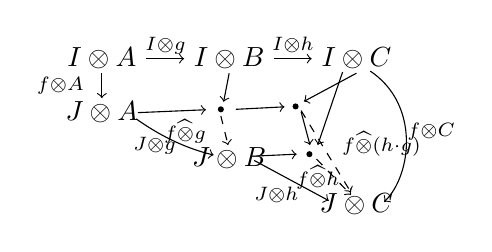
\begin{tikzpicture}[x=2.0em,y=1.5em]
  \node (IA) at (0,2.5) {$I\otimes A$};
  \node (IB) at (2.3,2.5) {$I\otimes B$};
  \node (IC) at (4.6,2.5) {$I\otimes C$};
  \node (JA) at (0,1.2) {$J\otimes A$};
  \fill (2.15,1.28) circle (1.1pt);
  \fill (3.5,1.35) circle (1.1pt);
  \node (JB) at (2.3,0.1) {$J\otimes B$};
  \fill (3.75,0.2) circle (1.1pt);
  \node (JC) at (4.6,-1.0) {$J\otimes C$};
  \draw[->] (IA) -- (IB);
  \node at (1.15,2.82) {$\scriptstyle I\otimes g$};
  \draw[->] (IB) -- (IC);
  \node at (3.45,2.82) {$\scriptstyle I\otimes h$};
  \draw[->] (0,2.15) -- (0,1.55);
  \node at (-0.75,1.85) {$\scriptstyle f\otimes A$};
  \draw[->] (0.65,1.2) -- (1.88,1.27);
  \draw[->] (2.3,2.15) -- (2.2,1.46);
  \draw[->] (4.6,2.15) -- (3.65,1.47);
  \draw[->] (2.42,1.28) -- (3.3,1.34);
  \draw[->,dashed] (2.15,1.12) -- (2.28,0.42);
  \node at (1.5,0.75) {$\scriptstyle f\widehat{\otimes}g$};
  \draw[->] (0.62,1.05) .. controls (1.2,0.5) and (1.7,0.28) .. (2.02,0.18);
  \node at (0.95,0.4) {$\scriptstyle J\otimes g$};
  \draw[->] (2.72,0.15) -- (3.52,0.2);
  \draw[->] (3.6,1.22) -- (3.76,0.42);
  \draw[->] (4.35,2.18) -- (3.9,0.42);
  \draw[->,dashed] (3.6,1.25) -- (4.5,-0.72);
  \node at (5.05,0.45) {$\scriptstyle f\widehat{\otimes}(h\cdot g)$};
  \draw[->,dashed] (3.88,0.08) -- (4.5,-0.78);
  \node at (3.9,-0.35) {$\scriptstyle f\widehat{\otimes}h$};
  \draw[->] (2.75,0.05) -- (4.1,-0.92);
  \node at (3.15,-0.78) {$\scriptstyle J\otimes h$};
  \draw[->] (4.85,2.2) .. controls (5.75,1.4) and (5.6,-0.3) .. (5.1,-0.95);
  \node at (5.95,0.75) {$\scriptstyle f\otimes C$};
  \node at (2.34,1.06) {$\lrcorner$};
  \node at (3.32,1.14) {$\lrcorner$};
  \node at (3.94,0.44) {$\lrcorner$};
\end{tikzpicture}
\end{center}
\item 胞腔复形结构：若 $f$ 与 $g$ 可分别表示为以 $f_{\alpha}$ 与 $g_{\beta}$ 为%
  \trCell{}的胞腔复形，且 $\otimes$ 在两个变量中都余连续，则 $f\widehat{\otimes}g$
  可表示为以 $f_{\alpha}\widehat{\otimes}g_{\beta}$ 为\trCell{}的胞腔复形。
\end{enumerate}
\end{proposition}

\begin{proof}
诸\trLeibnizProduct{}之间诱导结构同构的各分量皆是给定结构同构的实例，因而可逆，这
证明了 (i)。对于 (ii)，由定义双变量\trAdjunction{}
$(\otimes,\{,\},\mathrm{hom})$ 的诸\trIsomorphism{}之自然性，下方三个方块中
每一个可交换当且仅当另外两个可交换，其假设是在两幅图中取相同名称的水平箭头
互为转置：
\begin{center}
\begin{tikzpicture}[x=2.0em,y=1.75em]
  \node (P) at (0.9,1.4) {$J\otimes A\underset{I\otimes A}{\sqcup}I\otimes B$};
  \node (X) at (5.3,1.4) {$X$};
  \node (JB) at (0,0) {$J\otimes B$};
  \node (Y) at (5.3,0) {$Y$};
  \draw[->] (P) -- (X);
  \node at (3.1,1.76) {$\langle u,v\rangle$};
  \draw[->] (0,1.05) -- (0,0.35);
  \node at (-1.05,0.7) {$k\widehat{\otimes}\ell$};
  \draw[->] (5.3,1.05) -- (5.3,0.35);
  \node at (5.68,0.7) {$m$};
  \draw[->] (JB) -- (Y);
  \node at (2.65,-0.4) {$w$};
  \draw[->,dashed] (0.35,0.22) -- (5.0,1.18);
  \node at (1.8,0.9) {$x$};
  \node (A) at (8.0,1.4) {$A$};
  \node (JX) at (11.0,1.4) {$\{J,X\}$};
  \node (B) at (8.0,0) {$B$};
  \node (PB) at (11.6,0) {$\{J,Y\}\underset{\{I,Y\}}{\times}\{I,X\}$};
  \draw[->] (A) -- (JX);
  \node at (9.5,1.76) {$u$};
  \draw[->] (8.0,1.05) -- (8.0,0.35);
  \node at (7.63,0.7) {$\ell$};
  \draw[->] (11.15,1.05) -- (11.5,0.42);
  \node at (12.45,0.78) {$\widehat{\{k,m\}}$};
  \draw[->] (B) -- (PB);
  \node at (9.8,-0.44) {$\langle w,v\rangle$};
  \draw[->,dashed] (8.3,0.22) -- (10.85,1.2);
  \node at (9.4,0.95) {$x$};
\end{tikzpicture}
\end{center}
\begin{center}
\begin{tikzpicture}[x=2.1em,y=1.75em]
  \node (I) at (0,1.4) {$I$};
  \node (hBX) at (4.2,1.4) {$\mathrm{hom}(B,X)$};
  \node (J) at (0,0) {$J$};
  \node (PB) at (5.4,0) {$\mathrm{hom}(A,X)\underset{\mathrm{hom}(A,Y)}{\times}\mathrm{hom}(B,Y)$};
  \draw[->] (I) -- (hBX);
  \node at (2.1,1.76) {$v$};
  \draw[->] (0,1.05) -- (0,0.35);
  \node at (-0.42,0.7) {$k$};
  \draw[->] (4.75,1.1) -- (5.15,0.45);
  \node at (6.0,0.8) {$\widehat{\mathrm{hom}}(\ell,m)$};
  \draw[->] (J) -- (PB);
  \node at (2.35,-0.44) {$\langle u,w\rangle$};
  \draw[->,dashed] (0.35,0.22) -- (4.05,1.22);
  \node at (1.6,0.92) {$x$};
\end{tikzpicture}
\end{center}
这一转置对应可延伸到由这些方块所呈现的\trLifting{}问题的解上
（见\cref{ex:leibniz-lifting-equivalences}）。

性质 (iii) 是 $\widehat{\otimes}$ 在箭头\trCategory{}中的\trBifunctor{}性的
推论：任何\trBifunctor{}都保持收缩。性质 (iv) 几乎同样立即可得，因为%
\trCategoryOfArrows{}中的\trLimit{}与\trColimit{}皆按\trPointwise{}方式计算。
对于 (v)，考虑交换立方：
\begin{center}
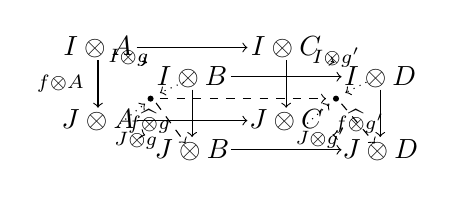
\begin{tikzpicture}[x=2.0em,y=1.32em]
  \node (IA) at (0,2.9) {$I\otimes A$};
  \node (IC) at (3.4,2.9) {$I\otimes C$};
  \node (IB) at (1.7,2.1) {$I\otimes B$};
  \node (ID) at (5.1,2.1) {$I\otimes D$};
  \node (JA) at (0,0.9) {$J\otimes A$};
  \node (JC) at (3.4,0.9) {$J\otimes C$};
  \node (JB) at (1.7,0.1) {$J\otimes B$};
  \node (JD) at (5.1,0.1) {$J\otimes D$};
  \fill (0.95,1.5) circle (1.1pt);
  \fill (4.3,1.5) circle (1.1pt);
  \draw[->] (IA) -- (IB);
  \node at (0.55,2.62) {$\scriptstyle I\otimes g$};
  \draw[->] (IC) -- (ID);
  \node at (4.3,2.62) {$\scriptstyle I\otimes g'$};
  \draw[->] (0.7,2.9) -- (2.7,2.9);
  \draw[->] (2.4,2.1) -- (4.4,2.1);
  \draw[->] (0,2.55) -- (0,1.25);
  \node at (-0.68,1.9) {$\scriptstyle f\otimes A$};
  \draw[->] (JA) -- (JB);
  \node at (0.68,0.36) {$\scriptstyle J\otimes g$};
  \draw[->] (0.7,0.9) -- (2.7,0.9);
  \draw[->] (2.4,0.1) -- (4.4,0.1);
  \draw[->] (1.7,1.75) -- (1.7,0.45);
  \draw[->] (3.4,2.55) -- (3.4,1.25);
  \draw[->] (5.1,1.75) -- (5.1,0.45);
  \draw[->] (JC) -- (JD);
  \node at (4.02,0.42) {$\scriptstyle J\otimes g'$};
  \draw[->,dotted] (1.55,1.95) -- (1.12,1.66);
  \draw[->,dotted] (0.4,0.82) -- (0.85,1.36);
  \draw[->,dashed] (1.05,1.38) -- (1.58,0.28);
  \node at (0.92,0.88) {$\scriptstyle f\widehat{\otimes}g$};
  \draw[->,dotted] (4.85,1.95) -- (4.47,1.66);
  \draw[->,dotted] (3.78,0.82) -- (4.18,1.36);
  \draw[->,dashed] (4.4,1.36) -- (5.0,0.28);
  \node at (4.72,0.88) {$\scriptstyle f\widehat{\otimes}g'$};
  \draw[->,dashed] (1.12,1.5) -- (4.12,1.5);
  \node at (1.18,1.64) {$\lrcorner$};
  \node at (4.52,1.64) {$\lrcorner$};
\end{tikzpicture}
\end{center}
由于 $I\otimes-$ 与 $J\otimes-$ 保持把 $g'$ 定义为 $g$ 之推出的那个推出，
立方的顶面与底面都是推出。定义诸\trLeibnizTensor{}之定义域的那些方块则在
左手面与右手面内部定义了推出。于是由推出的复合与消去即得所断言者：
$f\widehat{\otimes}g'$ 是 $f\widehat{\otimes}g$ 的一个推出。

(vi) 中展示的图式证明了那里所作的断言，故只剩下 (vii) 待证。首先注意：推出
的超限复合的推出仍是推出的超限复合，而超限复合的超限复合仍是超限复合，因此
只需逐个变量地工作，证明 $f\widehat{\otimes}-$ 保持 $g$ 的胞腔复形表示。为此，
设 $g$ 是诸映射 $g_i$ 的一个 $\alpha$-复合，其中每一个都是映射之余积
$g'_i=\coprod_{J}g'_{i,j}$ 的推出。我们可以把这个余极限提升到\trCategoryOfArrows{}%
中，将 $g=g_{0,\alpha}$ 视作\trDiagram{}
$g_{-,\alpha}\colon\alpha\to\mathcal{M}^{2}$ 的余极限，其单步映射为
\begin{center}
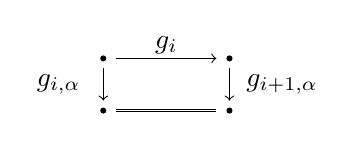
\begin{tikzpicture}[x=1.9em,y=1.45em]
  \fill (0,1.3) circle (1.1pt);
  \fill (2.4,1.3) circle (1.1pt);
  \fill (0,0) circle (1.1pt);
  \fill (2.4,0) circle (1.1pt);
  \draw[->] (0.25,1.3) -- (2.15,1.3);
  \node at (1.2,1.62) {$g_i$};
  \draw[->] (0,1.05) -- (0,0.25);
  \node at (-0.85,0.65) {$g_{i,\alpha}$};
  \draw[->] (2.4,1.05) -- (2.4,0.25);
  \node at (3.4,0.65) {$g_{i+1,\alpha}$};
  \draw[double] (0.25,0) -- (2.15,0);
\end{tikzpicture}
\end{center}

类似地，由 $g'_i$ 定义 $g_i$ 的那个推出方块可以提升为\trCategoryOfArrows{}中的
一个推出方块：
\begin{center}
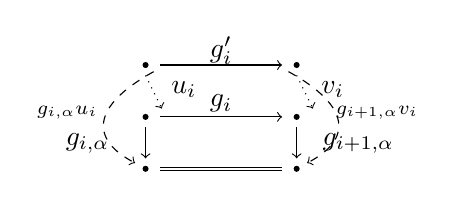
\begin{tikzpicture}[x=2.1em,y=1.5em]
  \fill (0,2.5) circle (1.1pt);
  \fill (2.6,2.5) circle (1.1pt);
  \fill (0,1.25) circle (1.1pt);
  \fill (2.6,1.25) circle (1.1pt);
  \fill (0,0) circle (1.1pt);
  \fill (2.6,0) circle (1.1pt);
  \draw[->] (0.25,2.5) -- (2.35,2.5);
  \node at (1.3,2.84) {$g'_i$};
  \draw[->] (0.25,1.25) -- (2.35,1.25);
  \node at (1.3,1.57) {$g_i$};
  \draw[double] (0.25,0) -- (2.35,0);
  \draw[->,dotted] (0,2.25) -- (0.28,1.45);
  \node at (0.66,1.9) {$u_i$};
  \draw[->,dotted] (2.6,2.25) -- (2.88,1.45);
  \node at (3.22,1.9) {$v_i$};
  \draw[->] (0,1.0) -- (0,0.25);
  \node at (-1.0,0.62) {$g_{i,\alpha}$};
  \draw[->] (2.6,1.0) -- (2.6,0.25);
  \node at (3.66,0.62) {$g_{i+1,\alpha}$};
  \draw[->,dashed] (0.14,2.34) .. controls (-0.95,1.5) and (-0.95,0.7) .. (-0.18,0.14);
  \node at (-1.35,1.35) {$\scriptstyle g_{i,\alpha}u_i$};
  \draw[->,dashed] (2.46,2.34) .. controls (3.55,1.5) and (3.55,0.7) .. (2.78,0.14);
  \node at (3.98,1.35) {$\scriptstyle g_{i+1,\alpha}v_i$};
  \node at (2.3,1.48) {$\lrcorner$};
\end{tikzpicture}
\end{center}
我们把这一立方诠释为：前面那个方块是后面那个方块的推出，而后者分解为相似
方块的余积——$g'_i=\coprod_{J}g'_{i,j}$ 的每个分量各对应一个。由此我们看出：
$g=g_{0,\alpha}$ 是某个\trDiagram{} $\alpha\to\mathcal{M}^{2}$ 之余极限的
定义域分量，这个\trDiagram{}的每一步都是\trCategoryOfArrows{}中映射之余积的
推出。现在 $f\widehat{\otimes}-\colon\mathcal{M}^{2}\to\mathcal{N}^{2}$ 保持%
\trCategoryOfArrows{}中的\trColimit，而定义域函子
$\mathrm{dom}\colon\mathcal{N}^{2}\to\mathcal{N}$ 也保持余极限。于是，
$f\widehat{\otimes}g$ 是诸映射 $f\widehat{\otimes}g'_{i,j}$ 之余积的推出的一个
$\alpha$-序列的余极限。

确立这些断言的更多细节见 \cite[\S4--\S5]{bib107}。
\end{proof}

\begin{definition}\label{def:left-leibniz-bifunctor}
设 $\mathcal{V}$、$\mathcal{M}$ 与 $\mathcal{N}$ 是余完备\trCategory，各自配备
弱分解系统 $(\mathrm{L},\mathrm{R})$、$(\mathrm{L}',\mathrm{R}')$ 与
$(\mathrm{L}'',\mathrm{R}'')$。一个\textbf{左 Leibniz \trBifunctor}（left
Leibniz bifunctor）是一个\trBifunctor{}
$\otimes\colon\mathcal{V}\times\mathcal{M}\to\mathcal{N}$，它
\begin{enumerate}[label=(\roman*)]
\item 在每个变量中分别余连续，并且
\item 具有\textbf{Leibniz 性质}（Leibniz property）：$\mathrm{L}$ 中一个映射
  与 $\mathrm{L}'$ 中一个映射的 $\otimes$-推出积落在 $\mathrm{L}''$ 中。
\end{enumerate}
\end{definition}

对偶地，配备弱分解系统的诸完备\trCategory{}之间的一个\trBifunctor{}是
\textbf{右 Leibniz \trBifunctor}（right Leibniz bifunctor），若它在每个变量中
分别连续，且右类中诸映射的拉回余张量落入右类。我们最常在\trBifunctor
\[ \{,\}\colon\mathcal{V}^{\mathrm{op}}\times\mathcal{N}\to\mathcal{M} \]
的情形下应用这一定义——它在其中一个变量上反变，此时相关的假设为：$\mathcal{V}$
余完备，且第一个变量中的余极限被携带为 $\mathcal{M}$ 中的\trLimit；此外，
$\mathrm{L}$ 中一个映射与 $\mathrm{R}''$ 中一个映射的\trLeibnizCotensor{}定义
$\mathrm{R}'$ 中的一个映射。左、右 Leibniz \trBifunctor{}之间的对偶性的本质
说起来颇为微妙，我们把它留作读者的一道谜题（或见 \cite{bib26}）。

\begin{lemma}\label{lem:leibniz-two-variable-adjunction}
若诸\trBifunctor
\[ \mathcal{V}\times\mathcal{M}\xrightarrow{\;\otimes\;}\mathcal{N},\qquad
   \mathcal{V}^{\mathrm{op}}\times\mathcal{N}\xrightarrow{\;\{,\}\;}
   \mathcal{M},\qquad\text{以及}\qquad
   \mathcal{M}^{\mathrm{op}}\times\mathcal{N}\xrightarrow{\;\mathrm{hom}\;}
   \mathcal{V} \]
定义一个双变量\trAdjunction，而 $(\mathrm{L},\mathrm{R})$、
$(\mathrm{L}',\mathrm{R}')$ 与 $(\mathrm{L}'',\mathrm{R}'')$ 分别是
$\mathcal{V}$、$\mathcal{M}$ 与 $\mathcal{N}$ 上的三个弱分解系统，则下列诸
条件等价：
\begin{enumerate}[label=(\roman*)]
\item $\otimes\colon\mathcal{V}\times\mathcal{M}\to\mathcal{N}$ 定义一个左
  Leibniz \trBifunctor；
\item $\{,\}\colon\mathcal{V}^{\mathrm{op}}\times\mathcal{N}\to\mathcal{M}$
  定义一个右 Leibniz \trBifunctor；
\item $\mathrm{hom}\colon\mathcal{M}^{\mathrm{op}}\times\mathcal{N}\to\mathcal{V}$
  定义一个右 Leibniz \trBifunctor。
\end{enumerate}
当这些条件成立时，我们说 $(\otimes,\{,\},\mathrm{hom})$ 定义一个
\textbf{Leibniz 双变量\trAdjunction}（Leibniz two-variable adjunction）。
\end{lemma}
\begin{proof}
伴随的存在保证每个\trBifunctor{}都满足所需的（余）连续性假设。注意，例如
$\mathrm{L}\widehat{\otimes}\mathrm{L}'\subset\mathrm{L}''$ 当且仅当
$\mathrm{L}\widehat{\otimes}\mathrm{L}'\llsq\mathrm{R}''$。于是三个陈述的%
等价由下述三个提升性质的等价得到：
\[ \mathrm{L}\widehat{\otimes}\mathrm{L}'\llsq\mathrm{R}''
   \quad\leftrightsquigarrow\quad
   \mathrm{L}'\llsq\widehat{\{\mathrm{L},\mathrm{R}''\}}
   \quad\leftrightsquigarrow\quad
   \mathrm{L}\llsq\widehat{\mathrm{hom}}(\mathrm{L}',\mathrm{R}''), \]
其证明留作\cref{ex:leibniz-lifting-equivalences}。
\end{proof}

\begin{remark}\label{rem:leibniz-generators}
由\cref{prop:leibniz-construction-preserves}(vii)，为证一个余连续\trBifunctor{}
$\otimes$ 满足 Leibniz 性质，只需证诸生成态射的 $\otimes$-\trLeibnizProduct{}落在陪域
弱分解系统的左类之中。
\end{remark}

\begin{lemma}\label{lem:set-tensor-leibniz}
对任何带积与余积、并配备弱分解系统 $(\mathrm{L},\mathrm{R})$ 的\trCategory{}
$\mathcal{M}$，集合张量、集合余张量与 hom
\[ \ast\colon\mathcal{S}et\times\mathcal{M}\to\mathcal{M},\qquad
   \{,\}\colon\mathcal{S}et^{\mathrm{op}}\times\mathcal{M}\to\mathcal{M},
   \qquad\text{以及}\qquad
   \mathrm{hom}\colon\mathcal{M}^{\mathrm{op}}\times\mathcal{M}\to\mathcal{S}et \]
相对于 $\mathcal{S}et$ 上的（\trMonomorphism，\trEpimorphism）弱分解系统
分别定义一个 Leibniz 双变量\trAdjunction。
\end{lemma}
\begin{proof}
由\cref{lem:leibniz-two-variable-adjunction}，只需证这些\trBifunctor{}中的
任何一个都是 Leibniz 的。当 $A\hookrightarrow B$ 是 $\mathcal{S}et$ 中的%
\trMonomorphism{}时，与 $f\colon X\to Y$ 的\trLeibnizTensor{}分解为显然落在
$\mathrm{L}$ 中的映射之余积：
\begin{rveq}\label{eq:set-tensor-leibniz-square}
\mbox{\begin{tikzpicture}[x=2.15em,y=1.55em]
  \node (AX) at (0,1.7) {$A\ast X$};
  \node (BX) at (4.6,1.7) {$B\ast X\cong A\ast X\sqcup B\setminus A\ast X$};
  \node (AY) at (0,0.2) {$A\ast Y$};
  \node (MY) at (4.6,0.2) {$A\ast Y\sqcup B\setminus A\ast X$};
  \node (BY) at (9.8,-0.35) {$B\ast Y\cong A\ast Y\sqcup B\setminus A\ast Y$};
  \draw[right hook->] (0.75,1.7) -- (2.0,1.7);
  \draw[->] (0,1.35) -- (0,0.55);
  \node at (-0.8,0.95) {$\scriptstyle A\ast f$};
  \draw[->] (4.6,1.35) -- (4.6,0.55);
  \node at (5.85,0.95) {$\scriptstyle A\ast f\sqcup\mathrm{id}$};
  \draw[->] (0.7,0.2) -- (2.6,0.2);
  \node at (3.5,0.46) {$\lrcorner$};
  \draw[->,dashed] (6.7,0.08) -- (7.85,-0.28);
  \node at (6.75,-0.56) {$\scriptstyle\mathrm{id}\sqcup B\setminus A\ast f$};
  \draw[->] (5.9,1.52) .. controls (8.1,1.25) and (9.6,0.65) .. (9.9,-0.02);
  \node at (8.35,0.98) {$\scriptstyle B\ast f$};
  \draw[->] (0.62,0.02) .. controls (3.0,-0.9) and (6.9,-1.0) .. (7.9,-0.5);
\end{tikzpicture}}
\end{rveq}
一个更利落的证明也是可能的。由于每个\trMonomorphism{}都可表示为由单个%
\trCell{} $\varnothing\hookrightarrow 1$ 构筑起来的胞腔复形，由%
\cref{prop:leibniz-construction-preserves}(vii)，只需考虑与生成\trMonomorphism{}
$\varnothing\hookrightarrow 1$ 的\trLeibnizTensor。但注意\trFunctor
\[ \mathcal{M}^{2}\xrightarrow{\;(\varnothing\hookrightarrow 1)\widehat{\ast}-\;}
   \mathcal{M}^{2} \]
自然\trIsomorphism{}于恒等\trFunctor，而后者当然保持左类 $\mathrm{L}$。
\end{proof}

\begin{remark}\label{rem:hom-right-leibniz}
由\cref{lem:set-tensor-leibniz}，
$\mathrm{hom}\colon\mathcal{M}^{\mathrm{op}}\times\mathcal{M}\to\mathcal{S}et$
是右 Leibniz 的，意即对任何 $\ell\in\mathrm{L}$ 与 $r\in\mathrm{R}$，态射
\[ \mathcal{M}(\mathrm{cod}\,\ell,\mathrm{dom}\,r)
   \xrightarrow{\;r\circ-\circ\ell\;}
   \mathcal{M}(\mathrm{dom}\,\ell,\mathrm{dom}\,r)
   \underset{\mathcal{M}(\mathrm{dom}\,\ell,\mathrm{cod}\,r)}{\times}
   \mathcal{M}(\mathrm{cod}\,\ell,\mathrm{cod}\,r) \]
是一个\trEpimorphism。这个映射的目标是 $\mathcal{M}$ 中从 $\ell$ 到 $r$ 的
交换方块之集，而其在任一元素上的\trFiber{}则是如此呈现的\trLifting{}问题之
解集。这一映射是\trEpimorphism{}这一事实重新表述了提升性质
$\mathrm{L}\llsq\mathrm{R}$。
\end{remark}

\subsection*{练习}

\begin{exercise}\label{ex:finish-closure-proof}
完成\cref{lem:right-lifting-closure}的证明。
\end{exercise}

\begin{exercise}\label{ex:retract-argument}
\begin{enumerate}[label=(\roman*)]
\item 证明「\trRetract{}论证」（retract argument）：设 $f=r\circ\ell$ 且 $f$
  对其右因子 $r$ 具有左\trLifting{}性质，则 $f$ 是其左因子 $\ell$ 的%
  \trRetract。
\item 据此得出：在\cref{def:weak-factorization-system}(i) 与 (ii) 存在时，
  (iii) 可代之以类 $\mathrm{L}$ 与 $\mathrm{R}$ 对收缩封闭这一假设。
\end{enumerate}
\end{exercise}

\begin{exercise}\label{ex:prove-adjunction-transposes}
证明\cref{lem:adjunction-transposes-lifting}。
\end{exercise}

\begin{exercise}\label{ex:inverse-category-diagram-wfs}
\begin{enumerate}[label=(\roman*)]
\item 设 $\mathcal{M}$ 是带\trProduct、\trPullback{}与塔之\trLimit{}的%
  \trCategory，配备弱分解系统 $(\mathrm{L},\mathrm{R})$。证明：对任何逆范畴
  $\mathcal{J}$，图表\trCategory{} $\mathcal{M}^{\mathcal{J}}$ 具有弱分解系统，
  其左类由诸分量皆为 $\mathrm{L}$ 中映射的映射组成，其右类由这样一些映射
  $\alpha\colon X\to Y$ 组成：对每个 $i\in\mathcal{J}$，相对匹配映射
  $\widehat{m}_i\colon X_i\to\partial_iX\underset{\partial_iY}{\times}Y_i$ 落在 $\mathrm{R}$ 中。
\item 在「$\mathcal{M}$ 的类 $\mathrm{F}$ 与 $\mathrm{F}\cap\mathrm{W}$ 是弱
  分解系统的右类」这一附加假设下，给出 $\lim\colon\mathcal{M}^{\mathcal{J}}\to\mathcal{M}$ 保持\trFibration{}与\trTrivialFibration{}的一个新证明。
\end{enumerate}
\end{exercise}

\begin{exercise}\label{ex:leibniz-lifting-equivalences}
给定双变量\trAdjunction{} \eqref{eq:two-variable-adjunction-functors} 与
$\mathcal{V}$、$\mathcal{M}$、$\mathcal{N}$ 中的映射类 $\mathrm{A}$、
$\mathrm{B}$、$\mathrm{C}$，证明下列提升性质等价：
\[ \mathrm{A}\widehat{\otimes}\mathrm{B}\llsq\mathrm{C}
   \quad\Leftrightarrow\quad
   \mathrm{B}\llsq\widehat{\{\mathrm{A},\mathrm{C}\}}
   \quad\Leftrightarrow\quad
   \mathrm{A}\llsq\widehat{\mathrm{hom}}(\mathrm{B},\mathrm{C}). \]
\end{exercise}

